\chapter{Timeline}
\label{ch:timeline}
% \vspace{-4em}
% \section{Timeline: 2020 - now}
% Before listing the timeline for the remainder of the project, let us first examine the timeline of the PhD so far: 
% %include the timeline PDF image here
% \begin{figure}[h!]
% \centering
% 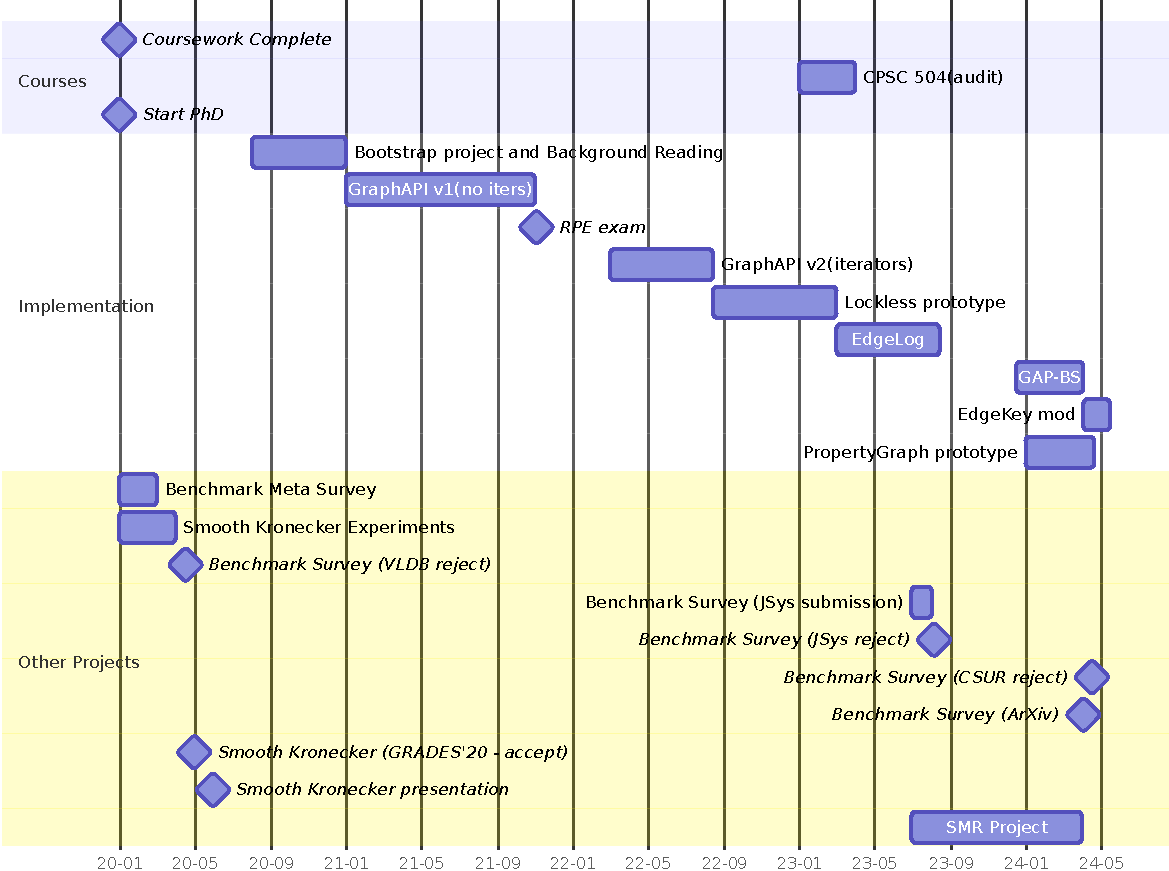
\includegraphics[scale=0.5,width=1.0\textwidth]{content/fig/timeline/past.mmd.pdf}
% \caption{Timeline 2020 - now}
% \label{fig:past-timeline}
% \end{figure}

% This timeline shows the major development phases for~\project{}.
% I started my PhD in January 2020 and submitted two papers between March and April 2020: one paper on the benchmarking practices common in graph processing systems research and another on the Smooth Kronecker Generator project from Daniel Margo's thesis~\cite{margo2017}.
% The Kronecker paper was published at GRADES-NDA 2020~\cite{10.1145/3398682.3399161}, and the benchmarking paper was rejected from VLDB 2020.
% I spent the remainder of 2020 adding more papers to read for the literature review and working on the benchmarking paper, while also trying to bootstrap the \project{} project.
% Alas, it was the year of the pandemic, and I was unable to make much progress on the project.

% I began working on the \project{} project in earnest in January 2021 and was able to finish the first version of the project by September 2021.
% I did my Research Proficiency Evaluation in November 2021 and passed.
% Following that, I traveled to India in December 2021 and got stuck there due to the Omicron variant.

% Upon my return in February 2022, I started working on the second version of the \project{} project.
% The second version included the redesigned API that was explicitly transactional and used iterators to access the data.
% We also tried to implement the use of edge-centric processing in the project, and while it is relatively straightforward to implement, it is not clear whether it will be beneficial.
% In Fall 2022, I worked on another feature that prototyped the use of lock-free data structures in the project, and some performance-related improvements around integer packing.

% In Spring 2023, I worked on the EdgeLog feature which was a new representation that used an insert-friendly log of edges as the primary representation; we abandoned this representation in favor of the improved EdgeKey representation that used fewer indices.

% In Fall 2023, I worked on revising and submitting the benchmarking paper to JSys, while also working on the SMR project and paper.
% The SMR paper was pushed to Spring 2024, and the benchmarking paper was desk rejected.

% In January 2024, I began fixing up the GraphAPI to be more usable and efficient. I also ported the \project{} to use the GAPBS kernel implementation.
% This was completed by April 2024, and I began working on the modified EdgeKey representation that does not use any indexes to access the edges.
% I also helped Jack with his project on inline property storage.
% Sometime in late March, I submitted the benchmarking paper to Computing Surveys, and it was rejected.
% It now lives on arXiv as a technical report~\cite{mehrotra2024sok}.

% \section{Timeline: Now - graduation}
\label{sec:future-timeline}
The timeline for the remainder of the project is shown in Figure~\ref{fig:future-timeline}.
Several tasks need to be completed before graduation.
The first, most important task is to put together a paper on the \project{} project.
We have already started working on this paper, and we expect to submit to VLDB 2025 on September 1st, 2024.

To evaluate~\project{} we need to compare it to other dynamic graph processing systems (\autoref{chapter:evaluation}) and to do that we need to finish the Grafaree project.
The Grafaree project is expected to be completed by the end of August 2024. 
While the Grafaree project is being completed, we will also be working on introducing the storage of labels and properties in \project{}.
The label and property storage project is expected to be completed by mid-October 2024, and I wish to submit the paper to VLDB 2026 on December 1st, 2025.

I would very much like to do an internship at a company or a research lab, and I am currently looking for opportunities.
I would ideally like to work on a project that is related to the \project{} project, but I am open to other ideas as well.
The internship would ideally be in the Spring of 2025, between January and May, giving me ample time to work on writing the dissertation and revise/resubmit the papers.

I wish to graduate in time for the November 2025 convocation and to do that, I need to have my thesis ready by the end of August 2025.
The timeline shown in Figure~\ref{fig:future-timeline} is based on the \href{https://www.grad.ubc.ca/current-students/final-doctoral-exam/doctoral-deadlines}{August 31st program end date doctoral deadline from G+PS}, but I am flexible with the exact date of graduation. 
The only hard deadline from G+PS is the dissertation submission deadline, which is July 26th, 2025; I would like to submit the dissertation much before then.

%include the timeline PDF image here
\begin{figure}[ht!]
\centering
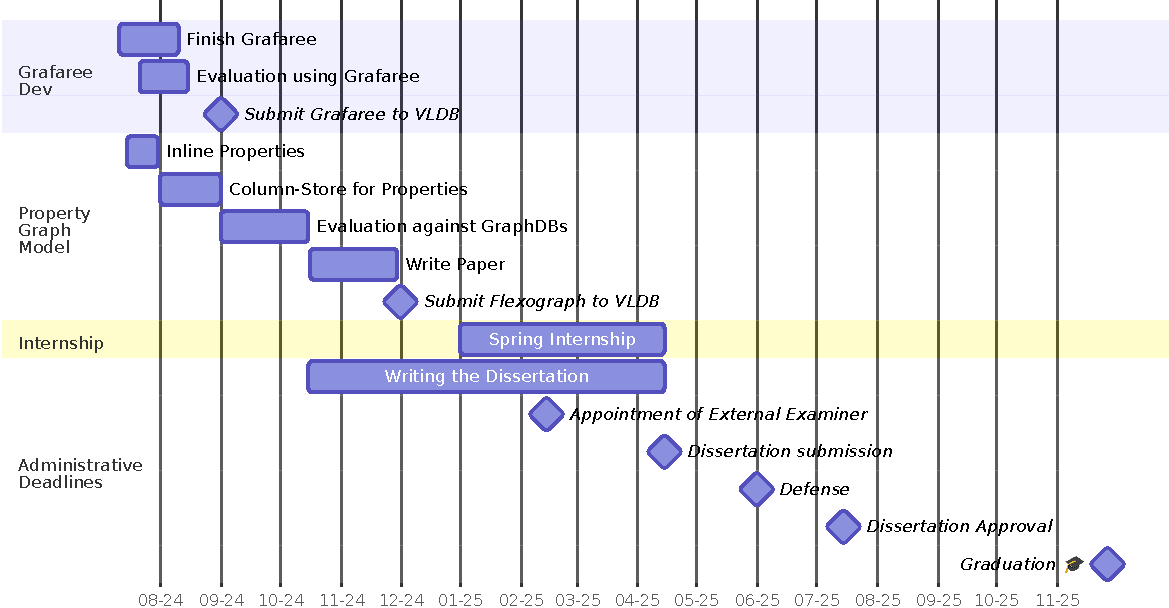
\includegraphics[width=1.0\textwidth]{content/fig/timeline/future.mmd.pdf}
\caption{Timeline between now until graduation}
\label{fig:future-timeline}
\end{figure}
